
\documentclass[]{article}
\usepackage{amsmath}
\usepackage{bm}
\usepackage{float}
\usepackage{amssymb}
\usepackage{listings}
\usepackage{mathtools}
\usepackage{tikz}

\DeclarePairedDelimiter\floor{\lfloor}{\rfloor}

\lstset{columns=fullflexible,
	mathescape=true,
	numbers=left,
	stepnumber=1,
	morekeywords={return, if, while, True, False},
	xleftmargin=5.0ex
}

\title{\vspace{-4.0cm}MAC0331 - Lista 4}
\author{Matheus T. de Laurentys, 9793714}

\begin{document}
	\maketitle
	\noindent
	\textbf{Q 8:} \\
	If using the definition of direction typical of the English language, the answer is no. The reason is that if a polygon is \mbox{$\alpha$-monotone}, then it is also \mbox{$(-\alpha)$-monotone}. If using the definition typical of the Portuguese, in which $\overline{NS}$ might mean $\overrightarrow{NS}$ or $\overleftarrow{NS}$ language, the answer is yes. 
	
	\textbf{Q 10:} \\
	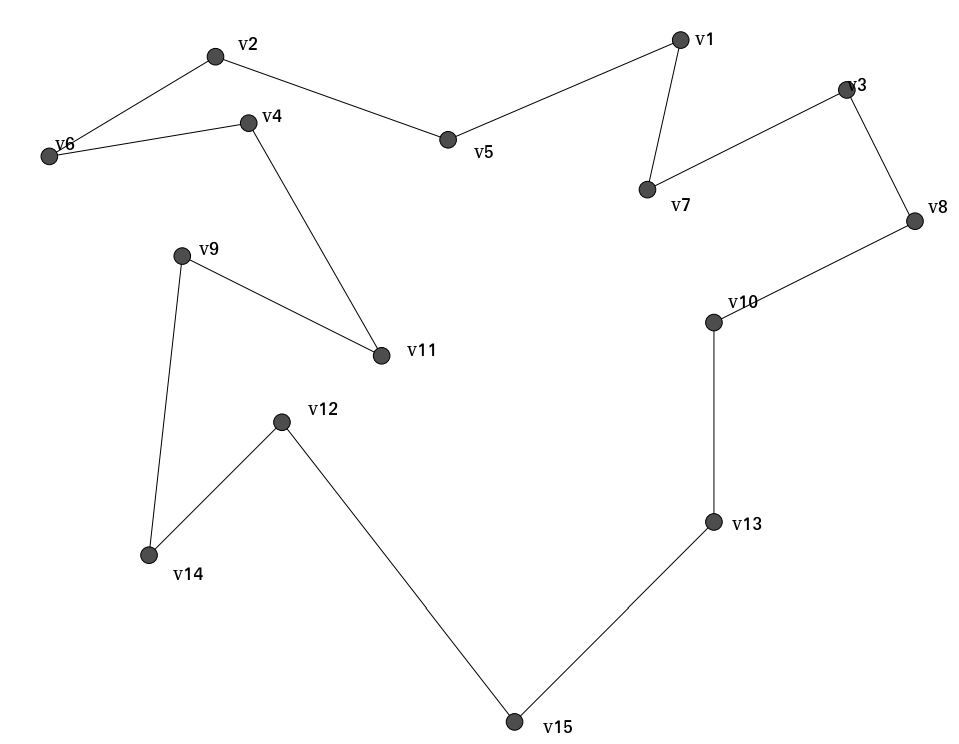
\includegraphics[scale=0.4]{l4_im.png} \\
	In the trace test, T is the sweep line and (c,v,d) is the set of the vertex analyzed and its left (c) and right (d) edges - those are not always named. D is the set of diagonals.
	\begin{table}[H]
	\begin{tabular}{lllll}
		Vertex & Case & Actions & D &  \\
		$v_1$ & 2 & T += (c,v,d) & {} &  \\
		$v_2$ & 2 & T += (c,v,d) & {} &  \\
		$v_3$ & 2 & T += (c,v,d) & {} &  \\
		$v_4$ & 2 & Replace trapeze with two new & {($v_2, v_4$)} &  \\
		$v_5$ & 3 & Replace two trapeze with one new & {($v_2, v_4$)} &  \\
		$v_6$ & 3 & Remove trapeze & {($v_2, v_4$)} &  \\
		$v_7$ & 3 & Replace trapeze with two new & {($v_2, v_4$), ($v_5, v_7$)} &  \\
		$v_8$ & 1 & Exchange trapeze & {($v_2, v_4$), ($v_5, v_7$), ($v_7, v_8$)} &  \\
		$v_9$ & 2 & T += (c,v,d) & {($v_2, v_4$), ($v_5, v_7$), ($v_7, v_8$)} &  \\
		$v_{10}$ & 1 & Exchange trapeze & {($v_2, v_4$), ($v_5, v_7$), ($v_7, v_8$)} &  \\
		$v_{11}$ & 3 & Replace two trapeze with one new & {($v_2, v_4$), ($v_5, v_7$), ($v_7, v_8$), ($v_5, v_{11}$)} &  \\
		$v_{12}$ & 2 & Replace trapeze with two new & ($v_2, v_4$), ($v_5, v_7$), ($v_7, v_8$), ($v_5, v_{11}$), ($v_{11}, v_{12})$) &  \\
		$v_{13}$ & 1 & Exchange trapeze & ($v_2, v_4$), ($v_5, v_7$), ($v_7, v_8$), ($v_5, v_{11}$), ($v_{11}, v_{12})$) &  \\
		$v_{14}$ & 3 & Remove trapeze & ($v_2, v_4$), ($v_5, v_7$), ($v_7, v_8$), ($v_5, v_{11}$), ($v_{11}, v_{12})$) &  \\
		$v_{15}$ & 3 & Remove trapeze & ($v_2, v_4$), ($v_5, v_7$), ($v_7, v_8$), ($v_5, v_{11}$), ($v_{11}, v_{12})$) & 
	\end{tabular}
	\end{table}
	
	$\textbf{Q15:}$\\
	a.
	\begin{lstlisting}
print_face_vertices (face f):
	start = f.edge
	n = start.next
	print(start.$v_0$)
	while (n != start):
		print(next.$v_0$)
		n = n.next
	\end{lstlisting}
	\begin{lstlisting}
print_adjacent_vertices(edge start): # start is (u,v) -- v is the target vertex
	e = start
	while (true):
		print(e.$v_0$)
		e = e.next.twin
		if (e == start):
			break
		
	\end{lstlisting}
\end{document}